\section{Probabilistic catalogs based on the 3FGL and 4FGL-DR2 catalogs}
\lb{sec:prob_cats}

In this section we use the ML algorithms optimized in the previous section to construct a probabilistic
classification of sources in the 3FGL and 4FGL-DR2 catalogs.



\subsection{Probabilistic classification of sources in 3FGL and comparison with 4FGL-DR2}
\lb{sec:3FGLprediction1}


We use the following four algorithms for the classification of sources: RF with 50 trees and maximal depth of 6, BDT with 100 trees and maximal depth of 2, NN with 11 neurons, LBFGS solver, and 300 epochs, and LR with LBFGS solver and 200 iterations. 
For training we use the pulsars and AGNs from the 3FGL catalog without missing or unphysical values. 
In addition to original datasets, we perform oversampling of pulsars in order to balance the numbers of pulsars and AGNs.
As a result, we have 8 classification methods: 4 algorithms trained with and without oversampling.


\begin{table}[!h]
\centering
\hspace{-0.2cm}
\resizebox{0.47\textwidth}{!}{
    \tiny
  \centering
    \renewcommand{\tabcolsep}{0.4mm}
\renewcommand{\arraystretch}{1.6}

%\hspace{-3mm}
    \begin{tabular}{c c c c c c c}
    \hline\hline
    Algorithm&Parameters &  Testing&Std. Dev.& Comparison with \\
    & & Accuracy & & 4FGL-DR2 Accuracy \\
    \hline
    RF & 50 trees, max depth 6  &97.37&0.60& 91.09 \\
    RF\_O &   &97.90&0.50& 89.44 \\
    \hline 
    BDT & 100 trees, max depth 2    &   97.65&0.54& 90.43 \\ 
    BDT\_O &     &   97.79&0.51& 91.75 \\
    \hline
    NN & 300 epochs, 11 neurons, LBFGS & 97.29&0.97& 90.10 \\
    NN\_O &  & 94.31&5.13& 87.13 \\
    \hline
    LR & 200 iterations, LBFGS solver & 97.63&0.54& 90.43 \\
    LR\_O &  &93.68&0.99& 85.15 \\
    \hline
     
    \end{tabular}}
    \vspace{2mm}
    \caption{Testing accuracy of the 4 selected algorithms for classification of 3FGL sources and comparison with associations in the 4FGL-DR2 catalog. 
    ``\_O'' denotes training with oversampling.}
    \label{tab:selected_algs}
\end{table}



\begin{figure}[h]
\centering
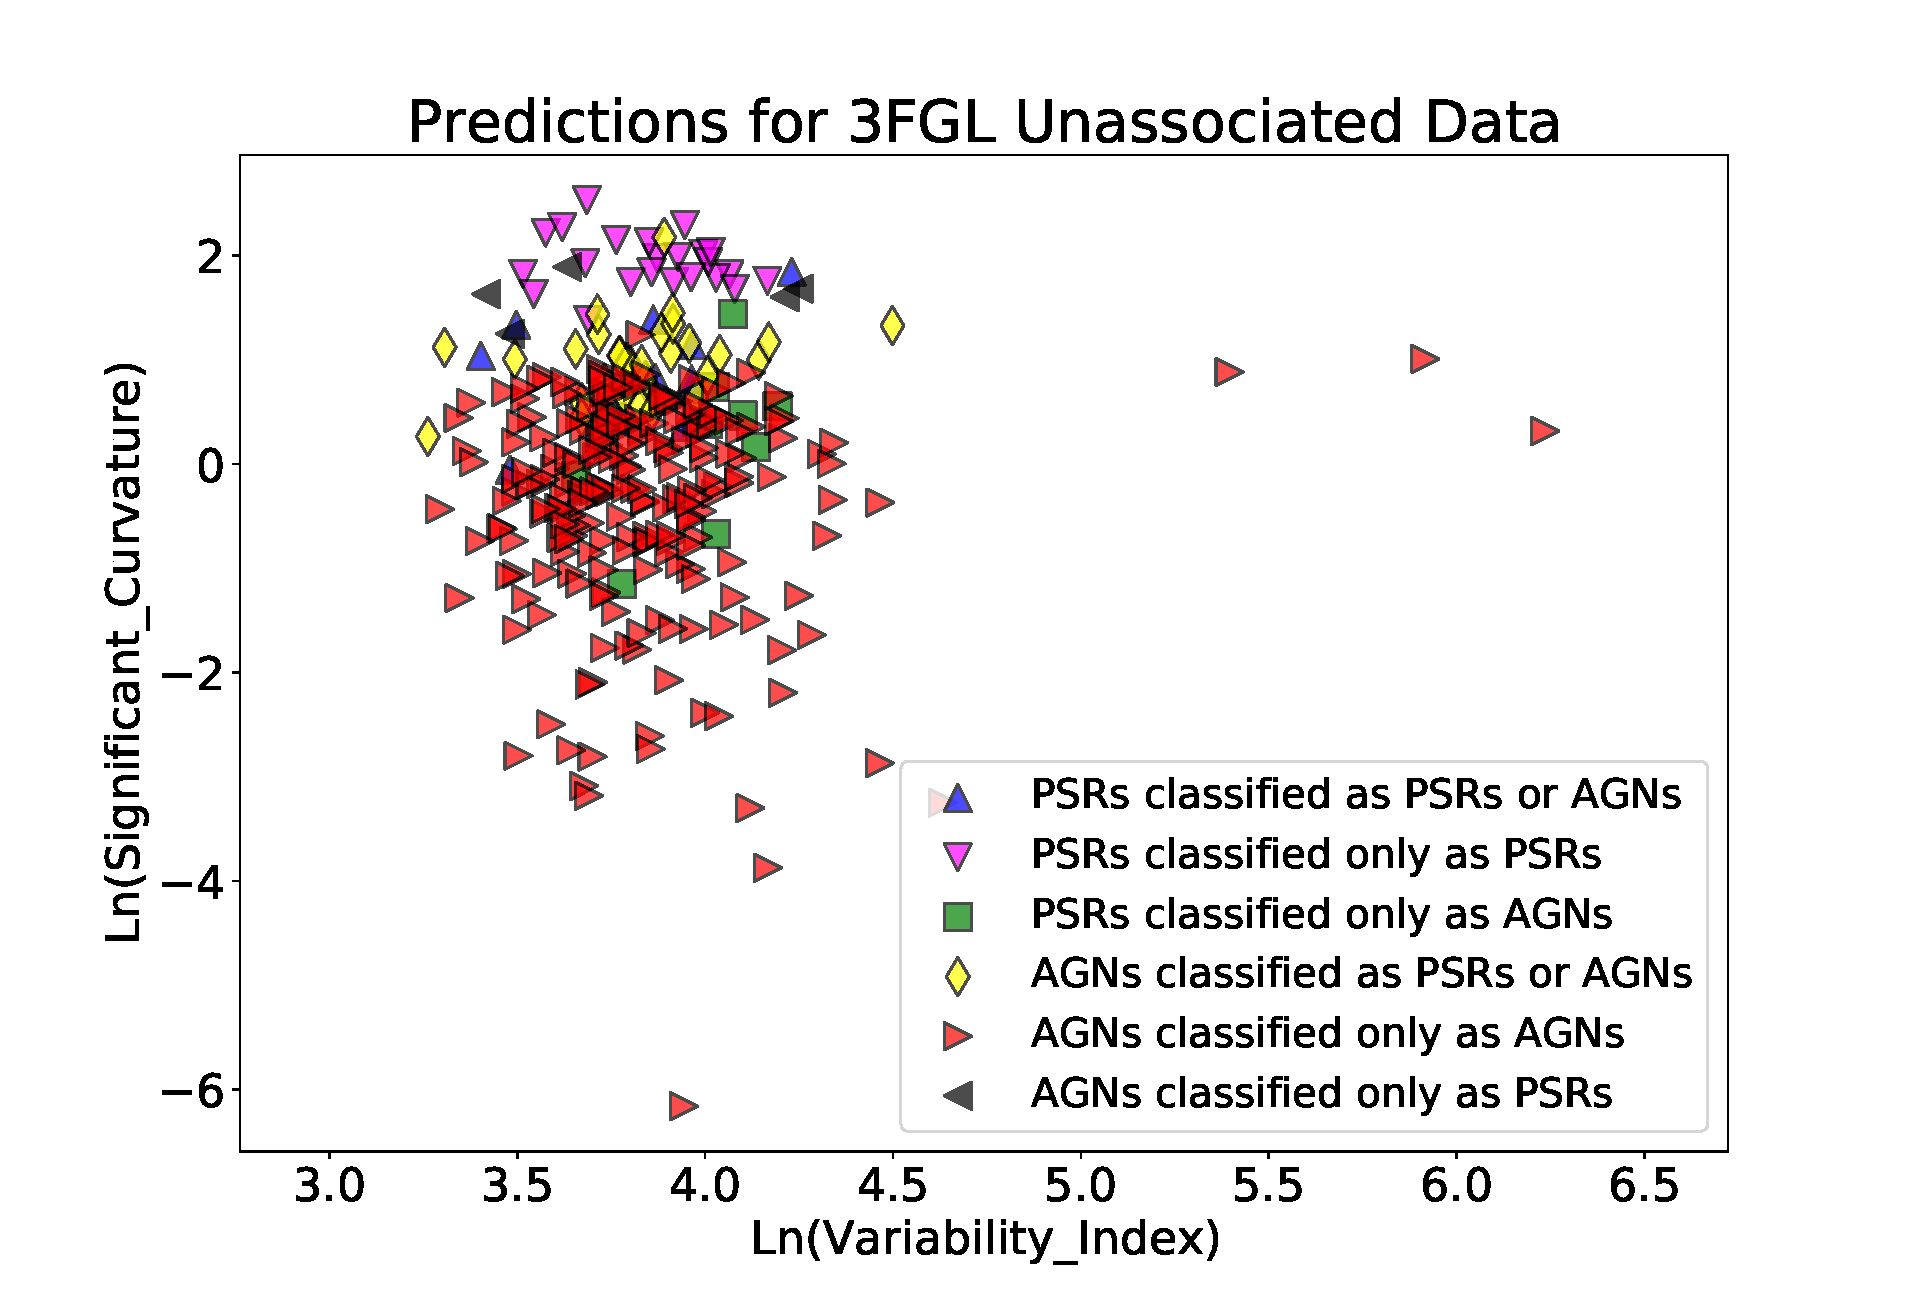
\includegraphics[width=0.48\textwidth]{plots/3FGL_unassoc_vs_4FGL-DR2_assoc.pdf}
\caption{Comparison of class prediction for unassociated 3FGL sources with classes in 4FGL-DR2. 
For more details see Section \ref{sec:3FGLprediction1}.}
\label{fig:3FGL_vs_4FGL_classes}
\end{figure}

The selected algorithms are summarized in Table \ref{tab:selected_algs}, where oversampling is shown by ``\_O''.
``Average testing accuracy'' is computed by taking 1000 times the 70\% - 30\% split into training and testing samples and averaging over the 
accuracies computed for the testing samples.
In addition, we look at sources, which are unassociated in 3FGL but have either pulsar or AGN association in 4FGL-DR2: there are 303 such sources.
The accuracy of our prediction for the four selected algorithms with and without oversampling, taking the 4FGL-DR2 classes as the true values, is reported in the column ``Comparison with 4FGL Accuracy''.
%The unassociated sources are classified as PSRs or AGNs by the individual ML algorithms, if the corresponding probability is larger than 0.5.

As a result of the classification with the eight ML methods,
we created a probabilistic catalog based on the 3FGL sources.
We train on 70\% of the sources associated with pulsars or AGNs without missing or unphysical values 
(there are thirteen sources with missing or unphysical values in the 3FGL catalog: 2 unassociated, 5 AGNs, 1 pulsar, and 5 ``other'' sources).
We replace the missing and unphysical values according to the procedure described at the beginning of Section \ref{sec:training}.
We calculate the probabilities of classes for testing sources, for sources which are not classified as pulsars or AGNs or have missing or unphysical values, and for unassociated sources.
We repeat the splitting and training 1000 times and report the sample average and standard deviation of the classification probabilities,
i.e., we average over 1000 values for unassociated sources, sources not classified as AGNs or pulsars, and sources with missing or unphysical values,
while the average for AGNs and pulsar without missing or unphysical values is over the number of times the sources appear in the testing sample, which is 300 on average.


In the probabilistic catalogs we add columns with corresponding probabilities for each algorithm and each class,
i.e., provided that there are 8 methods (including oversampling) and 2 classes, we add 16 columns: 8 for unweighted and 8 for oversampled training data. The columns with '\_O' represent the oversampled probabilities. We also add 16 columns for the standard deviations of probabilities. Although class probabilities and standard deviations for each algorithm are not independent (probabilities add up to 1 and standard deviations are equal for AGN and PSR classes), we keep the corresponding columns in view of the generalizations to multi-class classification (e.g., the 3-class classification in Section \ref{sec:3class}).

Table \ref{tab:prob_cat} shows an example of the probabilistic catalog for a few unassociated 3FGL sources.
Notice that the last source is classified as a pulsar by BDT and RF algorithms and as an AGN by LR and NN algorithms.
It is therefore an example of a source with mixed classification.


\pgfplotstableread[col sep=comma]{tables/3FGL_unassoc_vs_4FGL_assoc.csv}\loadedtable
\begin{table}
\centering
\pgfplotstabletypeset[columns={Source_Name_3FGL,AGN_BDT,AGN_RF,AGN_LR,AGN_NN},
column type=l,
string type,
every head row/.style={before row={\hline\hline & \multicolumn{4}{c}{AGN Probability} \\},after row=\hline,},
every last row/.style={after row=\hline}, %\vdots },
columns/Source_Name_3FGL/.style={column name=Source\_Name\_3FGL},
columns/AGN_BDT/.style={column name=BDT,numeric type,fixed,precision=3},
columns/AGN_NN/.style={column name=NN,numeric type,fixed,precision=3},
columns/AGN_RF/.style={column name=RF,numeric type,fixed,precision=3},
columns/AGN_LR/.style={column name=LR,numeric type,fixed,precision=3},
skip rows between index={4}{302}
]\loadedtable
\vspace{2mm}
\caption{\label{tab:prob_cat}
Example of the AGN classification probabilities for a few unassociated sources in the 3FGL catalog \citep{2015ApJS..218...23A}. 
We have omitted the oversampled probability columns here.}
\end{table}


%It can happen that different algorithms classify a source both as an AGN and as a pulsar.
For the determination of candidate classes based on the probabilistic classification, we consider the following two conditions:
1) that all algorithms agree, i.e., each algorithm predicts the same class for a source with more than 50\% probability,%
\footnote{We use the 50\% threshold in the 2-class case for illustration. Even if the probabilities for a source to be, e.g., a pulsar is larger than 50\% for all eight methods, there is still a large chance for the source to be an AGN if the probabilities are around 50\%. 
For this reason, the classes of sources reported in this work derived from the class probabilities should be viewed as candidate classes.
Depending on the application, a higher (lower) threshold can be used for a cleaner (more complete) sample. The full catalogs with all probabilities are available online \citep{SOM_material}.
More confident classification of particular sources can be obtained with multiwavelength studies, 
which are beyond the analysis in this paper.}
 and 
2) that the sum of probabilities for a source to belong to a certain class is larger than 7 
(this means that on average the probability is larger than 7/8 = 0.875).
Both of these conditions are stricter than the classification using probabilities for any of the 8 algorithms.
For convenience, we add a column in the probabilistic catalogs with the most likely probabilistic classes of sources based on the condition that all algorithms agree on the classification (sources with mixed classification are labeled as ``MIXED'' in this column).
In order to test the performance of the classification conditions we compare the precision and recall for unassociated source in the 3FGL catalog, which are associated in the 4FGL-DR2, and also calculate the expected precision and recall based on
test samples used in training.
In total there are 340 sources, which are unassociated in 3FGL but have associations in 4FGL-DR2.
The result of classification of the unassociated sources in the 3FGL catalog, which have associations in the 4FGL-DR2 catalog, 
using the condition that all methods agree on the classification are presented in Table~\ref{tab:3FGL_vs_4FGL_2class}.
``MIXED'' column shows the numbers of sources, for which different algorithms predict different classifications.
Columns show the predictions for the 3FGL unassociated sources, while the rows show the associations in the 4FGL-DR2 catalog.
For the later comparison with the 3-class classification, we also add unassociated source in the 3FGL catalog, 
which have associations with sources other than pulsars and AGNs.

We also present in Table~\ref{tab:3FGL_vs_4FGL_2class} the precision and recall estimates from the comparison of the 3FGL and 4FGL-DR2 catalogs (``4FGL assoc'' columns and rows).
For example, the precision for AGNs is the number of true positive predictions (223) over the number of positive predictions (the sum of numbers in the AGN column: (223 + 10 + 8), which gives $223 / 241 \approx 0.93$.
The estimated precision for PSRs is $ 23 / (23 + 5 + 6) \approx 0.68$.
In addition we show the expected precision and recall using the condition that all
methods agree (``all agree'' columns and rows) and the condition that the sum of probabilities is larger than 7 (``$\sum_a p_a > 7$'' columns and rows) calculated using the class probabilities for associated sources reported in the probabilistic catalogs (these probabilities are derived as an average over the test samples).
The precision (recall) estimates using, e.g., the condition that all algorithms agree is computed by taking the ratio of associated pulsars in 3FGL, which are also predicted to be pulsars by all 8 algorithms, to the number of sources associated with pulsars (to the total number of sources predicted to be pulsars among associated sources) in the 3FGL catalog.
The precision and recall estimates for the $\sum_a p_a > 7$ condition are computed analogously.
The latter condition is on average stricter than the ``all agree'' condition, which results in larger precision and smaller recall than in the ``all agree'' case.
Also all unassociated 3FGL pulsar candidates, which satisfy $\sum_a p_a > 7$ condition, are associated to pulsars in the 4FGL-DR2.

We note that the precision and recall with the ``all agree'' condition from the comparison of 3FGL and 4FGL-DR2 catalogs is worse than the precision and recall expectations using the estimates from the test samples in training.
In order to understand the reason for the worse performance of classification in comparison of 3FGL predictions with the 4FGL-DR2 associations relative to the expectations we plot in Fig.~\ref{fig:3FGL_vs_4FGL_classes} the 303 sources unassociated in 3FGL but with PSR or AGN associations in 4FGL-DR2.
The class at the beginning of the label name in Fig.~\ref{fig:3FGL_vs_4FGL_classes} corresponds to the association in the 4FGL-DR2, while the second half of the labels corresponds to classification of unassociated sources in 3FGL. For example, ``PSRs classified only as PSRs'' shows sources which have a PSR association in 4FGL-DR2 and all eight methods classified the corresponding unassociated sources in 3FGL as a pulsar. ``PSRs classified as either PSRs or AGNs'' labels sources with PSR associations in 4FGL-DR2 but the corresponding unassociated sources in 3FGL have both PSR and AGN classifications by different ML methods.
We notice that misclassified or partially misclassified sources in Fig. \ref{fig:3FGL_vs_4FGL_classes} typically happen on the boundary between the two classes or even inside the opposite class.
Many of these sources also have flags in the 3FGL catalog, such as a potential problem with the background diffuse emission model in the location of the source, which can lead to a poor reconstruction of the source spectrum and, consequently, misclassification of the source.
The estimated precision for AGNs (pulsars) using either ``all-agree'' or $\sum_a p_a > 7$ condition is better than about 97\% (80\%) with the 2-class classification, while the precision estimates from the comparison of 3FGL and 4FGL-DR2 catalogs is about 93\% (70\%) for AGNs (pulsars).
We will see in Section \ref{sec:3class} that the expected precision using  either ``all-agree'' or $\sum_a p_a > 7$ condition for the 3-class classification for AGNs (pulsars) is better than about 99\% (90\%), but the precision estimated from the comparison of 3FGL and 4FGL-DR2 catalogs is still about 93\% (70\%).
Thus even if the expected precision is better in the 3-class case than in the 2-class case, the precision estimates from the comparison of 3FGL and 4FGL-DR2 catalogs are similar in the 2- and 3-class cases.
We conclude that the smaller precision in the comparison of the 3FGL and 4FGL-DR2 catalogs is mostly due to errors and uncertainties in the input data and represents an irreducible error of the analysis.


%
%\dima{new text: Overall there are 275 sources in Table \ref{tab:3FGL_vs_4FGL_2class} classified as pulsars or AGNs by all 8 methods. Among these sources, 246 have correspondingly pulsar or AGN associations in the 4FGL-DR2 catalog, while the remaining 29 sources were misclassified, which can be interpreted as 10.5\% false positive rate. This false positive rate is consistent with about 90\% accuracy for the individual methods.}


\begin{table}[!h]
\centering
\resizebox{0.47\textwidth}{!}{
    \tiny
  
 \renewcommand{\tabcolsep}{0.3mm}
\renewcommand{\arraystretch}{1.5}

    \begin{tabular}{l c c c c c c}
    \hline
    \hline
    4FGL-DR2 class & \multicolumn{3}{c}{3FGL prediction} \ &  Recall\ \ & Recall & Recall\\
      &\ AGN &\ PSR &\ MIXED & (4FGL assoc) & (all agree) & ($\sum_a p_a > 7$) \\
    \hline
    AGN & 223 & 5 &  30 & 0.86 & 0.94 & 0.92 \\ % 258
    PSR & 10 & 23 &  12  & 0.51 & 0.67 & 0.61 \\ % 45
    OTHER & 8 & 6 & 23  & -- & -- & --\\ % 37
    \hline
    Precision (4FGL assoc) & 0.93 & 0.68 & --  \\
    Precision (all agree) & 0.97 & 0.78 & --  \\
    Precision ($\sum_a p_a > 7$) & 0.98 & 0.82 & --  \\
    \hline
    \end{tabular}}
    \vspace{2mm}
    \caption{
    Comparison of classes predicted for unassociated sources in the 3FGL catalog using 2-class classification
    with associations in the 4FGL-DR2 catalog. 
    The precision and recall are calculated using all-algorithms-agreement condition and 4FGL-DR2 associations (``4FGL assoc'' labels)
    or the class probabilities of associated 3FGL sources derived from test samples using either all-algorithms-agreement condition (``all agree'' labels) or the $\sum_a p_a > 7$ condition (``$\sum_a p_a > 7$'' labels).
    The AGN and PSR sources are also represented in Fig. \ref{fig:3FGL_vs_4FGL_classes}.}
    \label{tab:3FGL_vs_4FGL_2class}
\end{table}








\begin{table}[!h]
\centering
\resizebox{0.4\textwidth}{!}{
    \tiny
    \renewcommand{\tabcolsep}{0.3mm}
\renewcommand{\arraystretch}{1.5}

    \begin{tabular}{l  l c c c c}
    \hline
    \hline
    Catalog & Classification &\ AGN &\ PSR &\ OTHER &\ MIXED \\
    \hline
    3FGL & 2-class & 599 & 111 & --  &  300 \\
     & {2-class corr} & { 580.0} & { 97.0} & { 56.4}  &  { 276.5} \\
     & 3-class & 587 & 53 & 69  &  301 \\
    \hline
    4FGL-DR2 \ & 2-class & 878 & 162 & --  &  627 \\
     & {2-class corr} & {826.2} & { 134.5} & { 140.4}  &  {565.9} \\
     & 3-class & 739 & 64 & 274  &  590 \\
    \hline
     
    \end{tabular}}
    \vspace{2mm}
    \caption{Expected number of AGNs, pulsars, and other sources as well as sources with mixed classifications
    among the unassociated 3FGL and 4FGL-DR2 sources derived with the 2-class (Section \ref{sec:prob_cats}) 
    and 3-class (Section \ref{sec:3class}) classification.
    The ``2-class corr'' row shows correction of the 2-class classification prediction due to the presence of OTHER sources among 
    the unassociated ones (see Section \ref{sec:3FGLprediction1} for details).}
    \label{tab:prediction_2and3class}
\end{table}



We summarize the results of classification of unassociated 3FGL sources with the 2-class classification 
in Table \ref{tab:prediction_2and3class} in the 3FGL ``2-class'' row.
The ``AGNs'' column shows the number of unassociated sources predicted to be AGNs using the all-algorithms-agree condition.
Similarly the ``Pulsars'' column shows the number of unassociated sources where all the algorithms predict the source to more likely be a pulsar.
The ``Mixed'' column shows the number of sources with mixed classification, i.e., some algorithms predict that the source is more likely an AGN while the other algorithms predict that it is more likely a pulsar.
We also add the ``OTHER'' column in order to compare the results with the 3-class classification in Section \ref{sec:3class}.
Since there is no ``OTHER'' class in the 2-class classification, the corresponding entry is empty.
Out of 1010 unassociated sources in 3FGL, 111 are classified as pulsars by all eight methods, 599 are classified as AGNs, and 300 have mixed classifications.



In the ``2-class corr'' row of Table \ref{tab:prediction_2and3class}
we show a possible correction of the number of pulsars and AGNs due to the presence of other sources.
Here we assume that the fraction of AGN-like and pulsar-like sources among the other sources is the same for associated and for unassociated sources.
In particular, if we denote by $N_{\rm AGN}$ the number of unassociated sources with AGN-like probabilistic classification,
by $N_{\rm AGN}^{\rm ass\,OTHER}$ the number of sources with AGN-like classification among associated OTHER sources,
by $N_{\rm ass}$ ($N_{\rm unass}$) the total number of associated (unassociated) sources, then
the number of AGN-like sources among the unassociated ones corrected for the presence of OTHER sources can be estimated as
\bea
\lb{eq:other_correction}
N_{\rm AGN}^{\rm corr} = N_{\rm AGN} - N_{\rm AGN}^{\rm ass\,OTHER} \,\frac{N_{\rm unass}}{N_{\rm ass}}.
\eea
Analogous corrections are applied for the number of unassociated sources with PSR and with mixed classifications.
If we denote by $N^{\rm ass\,OTHER}$ the total number of associated other sources, then the estimated number of 
OTHER sources among unassociated ones is
\bea
\lb{eq:2class_other}
N^{\rm unass}_{\rm OTHER} = N^{\rm ass\,OTHER} \,\frac{N_{\rm unass}}{N_{\rm ass}}.
\eea
We show this estimate in the OTHER column in the ``2-class corr'' row.
We note that since 
$N_{\rm AGN}^{\rm ass\,OTHER} + N_{\rm PSR}^{\rm ass\,OTHER} + N_{\rm MIXED}^{\rm ass\,OTHER} = N^{\rm ass\,OTHER}$,
this estimate is consistent with corrections in Eq. (\ref{eq:other_correction}) for sources classified as AGNs, pulsars, or with mixed classification.







\subsection{Probabilistic classification of sources in the 4FGL-DR2 catalog}
\lb{sec:4FGLprediction}

In this section we construct a probabilistic classification of sources in the 4FGL-DR2 catalog. The 4FGL-DR2 catalog \citep{2020arXiv200511208B} 
is based on 10 years of \Fermi-LAT data \citep[compared to 8 years of data in the 4FGL catalog,][]{2020ApJS..247...33A}.
It contains 5788 sources, which is 723 sources more than in the 4FGL catalog (all sources in 4FGL are kept in 4FGL-DR2 even if they fall
below the detection threshold with 10 years of data). 
In the 4FGL-DR2 catalog,
3503 sources are associated to AGNs,
271 sources are associated to pulsars,
1658 sources are unassociated (we only look at CLASS1 column in the catalog), 
and the rest 346 sources are other sources, such as PWN, SNR, etc.
There are 14 sources in 4FGL-DR2 with missing or unphysical values: four AGNs, one PWN (Crab), and nine unassociated sources.
As in the previous section, we use sources associated with either AGNs or pulsars for training,
which have no missing or unphysical values.
The unphysical and missing values are replaced according to the procedure described at the beginning of Section \ref{sec:training}.
We calculate the classification probabilities of AGN and PSR classes for both the associated and the unassociated sources.

The 4FGL-DR2 catalog has a higher number of features, especially due to the difference in modeling of the spectra compared with the 3FGL catalog. 
We selected 28 of these features plus 6 hardness ratios HR12, ..., HR67 (the 4FGL-DR2 catalog has 7 energy bins)
and looked for correlations among them. 

If any feature was correlated or anti-correlated with a Pearson index of $\pm$0.75 or higher with another feature, then only one of these features was kept. 
The resulting 16 features are:
GLON, GLAT, ln(Pivot\_Energy), ln(Energy\_Flux100), ln(Unc\_Energy\_Flux100), LP\_Index, Unc\_LP\_Index, LP\_beta, LP\_SigCurv, ln(Variability\_Index), and the 6 hardness ratios.

For the classification of 4FGL-DR2 sources, we confirmed that the parameters used in 3FGL classification provide an optimal performance also for the 4FGL-DR2 catalog, except for NN, which requires more neurons in the hidden layer in the 4FGL-DR2 case.
Therefore, we used the same meta-parameters for the four algorithms as in the construction of the probabilistic catalog based on 3FGL, except for NN where we increased the number of neurons in the hidden layer to 16. Similar to the construction of the 3FGL probabilistic catalog, we use both unweighted training samples and oversampling, i.e., we have 8 classification methods.
We retrain the algorithms using the 16 features for the 4FGL-DR2 sources.
The corresponding accuracies are reported in Table \ref{tab:selected_algs2}.



\begin{table}[!h]
\centering
%\resizebox{0.45\textwidth}{!}{
    \tiny
    \renewcommand{\tabcolsep}{0.4mm}
\renewcommand{\arraystretch}{1.6}

    \begin{tabular}{ c c c c }
    \hline
    \hline
    Algorithm&Parameters &  Testing&Std. Dev.\\
    & & Accuracy\ &  \\
    \hline
    RF& 50 trees, max depth 6  &97.87 & 0.36\\
    RF\_O   &&97.56&0.39 \\
    \hline
    BDT & 100 trees, max depth 2    &   97.63 &0.39\\
    BDT\_O&&97.72&0.38\\
    \hline
    NN & 300 epochs, 16 neurons, LBFGS  & 97.41 & 0.47\\
    NN\_O&&95.48&0.66\\
    \hline
    LR & 200 iterations, LBFGS solver & 97.80&0.38\\
    LR\_O&&96.03&0.53\\
    \hline
     
    \end{tabular}%}
    \vspace{2mm}
    \caption{Testing accuracy of the 4 algorithms on 4FGL-DR2 associated data. ``\_O'' denotes training with oversampling.}
    \label{tab:selected_algs2}
\end{table}


\begin{table}[!h]
\centering
%\resizebox{0.47\textwidth}{!}{
    \tiny
  
 \renewcommand{\tabcolsep}{0.3mm}
\renewcommand{\arraystretch}{1.5}

    \begin{tabular}{l c c c c}
    \hline
    \hline
    & classification &\ \  AGN &\ \   PSR &\ \   OTHER \\
    \hline
    2-class precision & all     agree            & 0.96 &  0.71 & --  \\ 
                                & $\sum_a p_a > 7$ & 0.97 &  0.78  & -- \\
    \hline
    2-class recall       & all     agree            & 0.95 &  0.70 & --  \\ 
                                & $\sum_a p_a > 7$ & 0.94 &  0.64  & -- \\
    \hline
    3-class precision & all     agree            & 0.98 & 0.89  & 0.80  \\ 
                                & $\sum_a p_a > 7$ & 0.99 &  0.94  & 0.85 \\
    \hline
    3-class recall       & all     agree            & 0.94 &  0.62 & 0.38  \\ 
                                & $\sum_a p_a > 7$ & 0.87 &  0.30  & 0.06 \\
    \hline
    \end{tabular}%}
    \vspace{2mm}
    \caption{The expected precision and recall for the classification of 4FGL-DR2 sources
    for two classification conditions: all algorithms agree (``all agree'' rows) and that the sum of probabilities for the 8 algorithms 
    is larger than 7 (``$\sum_a p_a > 7$'' rows). For details on the 2- and 3-class classification see Sections \ref{sec:4FGLprediction} and 
    \ref{sec:3class} respectively. }
    \label{tab:prec_recall_4FGL}
\end{table}

Analogously to the 3FGL catalog, we use the agreement among the algorithms for the probabilistic classification of sources.
We report the corresponding precision and recall in Table \ref{tab:prec_recall_4FGL}, where we also show precision and recall
for the $\sum_a p_a > 7$ condition and for the 3-class classification described in Section \ref{sec:3class}.
Using the agreement among the algorithms condition,
we calculate the expected numbers of pulsars and AGNs among the 1658 unassociated sources in 4FGL-DR2 without missing values 
(see 4FGL-DR2 part of Table \ref{tab:prediction_2and3class}).
The definition of rows is the same as in the 3FGL catalog 2-class classification in Section \ref{sec:3FGLprediction1}.

Finally, we looked at sources which were unassociated in both 3FGL and 4FGL-DR2 (using 'ASSOC\_FGL' as an identifier for 3FGL sources). Out of 303 such sources%
\footnote{The 303 unassociated 4FGL-DR2 sources correspond to 302 unassociated 3FGL sources, because there are two 4FGL-DR2 sources, which are associated with one 3FGL source.},
40 sources are predicted to be pulsars using 3FGL features and 75 sources are predicted to be pulsars using 4FGL-DR2 features. This leads to 29 sources which are predicted by all eight methods to be pulsars for features taken from both the 3FGL and 4FGL-DR2 catalogs. 
For convenience, we save these 29 pulsar candidates as a separate file (``3FGL\_4FGL-DR2\_Candidates\_PSR.csv'' in the supplementary online materials \citep{SOM_material}). Out of these 29 sources classified as pulsars, 4 sources have counterparts in Parkes survey \citep{Camilo2015} within 2 arc minutes (see Table \ref{tab:parkes}). The data for the Parkes association candidates is also added to the ``3FGL\_4FGL-DR2\_Candidates\_PSR.csv'' file.

\pgfplotstableread[col sep=comma]{tables/3fgl_unassoc_predictions_matches_with_Parkes_2015_1.csv}\loadedtable
\begin{table}[h]
\centering
\pgfplotstabletypeset[columns={Source_Name_4FGL,GLON_4FGL,GLAT_4FGL,Separation_Parkes},
column type=l,
string type,
every head row/.style={before row={\hline \hline},after row=\hline,},
every last row/.style={after row=\hline},
columns/Source_Name_4FGL/.style={column name=Source\_Name\_4FGL},
columns/GLON_4FGL/.style={column name=GLON,numeric type,fixed,precision=1},
columns/GLAT_4FGL/.style={column name=GLAT,numeric type,fixed,precision=1},
columns/Separation_Parkes/.style={column name=Sep (arcsec),numeric type,fixed,precision=1}
]\loadedtable
\vspace{2mm}
\caption{\label{tab:parkes}
Connection of unassociated 3FGL and 4FGL-DR2 sources classified as pulsars with Parkes pulsars \citep{Camilo2015}. GLON and GLAT are taken from 4FGL-DR2 and the separations in arcseconds with Parkes pulsars are given in the ``Sep (arcsec)'' column.}
\end{table}






